\begin{figure}
\centering

\ifpdf
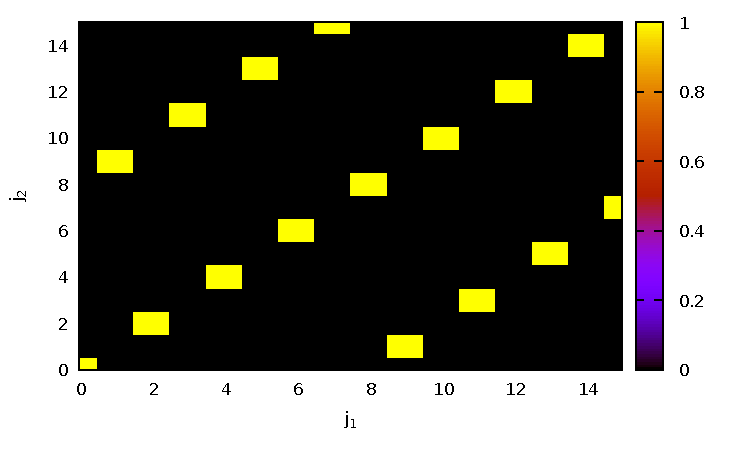
\includegraphics[angle=0]
{./discretlog/picdiscretlog2.pdf}
\else
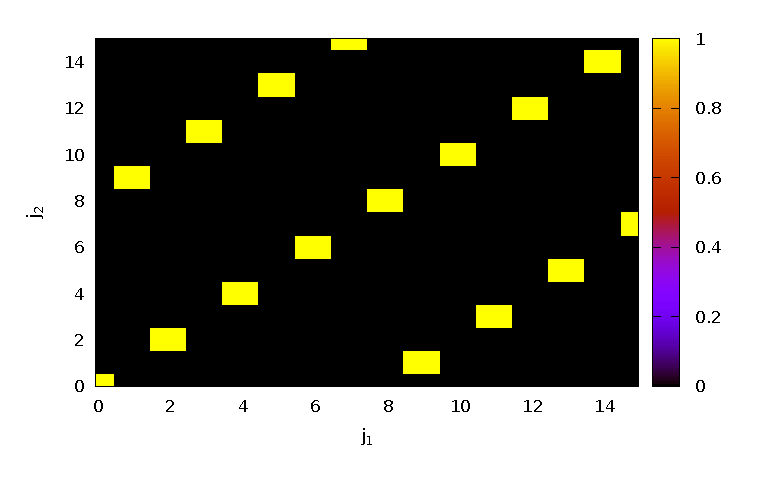
\includegraphics[angle=0]
{./discretlog/picdiscretlog2.eps}
\fi

%\input ./discretlog/picdiscretlog2.tex

\caption{Fourier transform of the function from \autoref{fig:dl1}.
  Number of samples $M=16$. Coordinates of the maximum $j_1 = 9$, $j_2 = 1$. 
The solution of the equation $3^x \equiv 14 \mod 17$
is $x \equiv 9 \cdot 1^{-1} \equiv 9 \mod 16$. Considering that
the period is less than the number of samples, we can conclude that $x = 9$} 
\label{fig:dl2}
\end{figure}
